\documentclass[twoside]{article}
\usepackage[utf8]{inputenc}
\usepackage{amsmath,amsfonts,amssymb,amsthm,latexsym}
\usepackage[spanish,es-noshorthands]{babel}
\usepackage[T1]{fontenc}
\usepackage{lmodern}
\usepackage{graphicx,hyperref}
\usepackage{tikz,pgf}
\usepackage{marvosym}
\usepackage{multicol}
\usepackage{fancyhdr}
\usepackage[papersize={5.5in,8.5in},left=.75cm,right=.75cm,top=1.5cm,bottom=1.25cm]{geometry}
\usepackage{fancyhdr}
\pagestyle{fancy}
\fancyhead[LE]{Colegio Arborizadora Baja}
\fancyhead[RE]{PEI:``Hacia una cultura para el desarrollo sostenible''}
\fancyfoot[RO]{\Email gavendanor@colarborizadorabaja.edu.co}
\fancyhead[LO]{\url{www.autistici.org/mathgerman}}
\fancyfoot[RE]{\Email cedarborizadoraba19@redp.edu.co}
\fancyfoot[LE]{Calle 59I \#44A - 02 \Telefon 7313994-7313995}
\fancyhead[RO]{Nit 830024976-8, Código DANE 11100103084-8}

\author{Germ\'an Avenda\~no Ram\'irez~\thanks{Lic. Mat. U.D., M.Sc. U.N.}}
\title{\begin{minipage}{.2\textwidth}

\includegraphics[height=1.75cm]{Images/logo-colegio.png}\end{minipage}
\begin{minipage}{.55\textwidth}
\begin{center}
Números racionales $\mathbb{Q}$\\
Matemáticas $9^{\circ}$
\end{center}
\end{minipage}\hfill
\begin{minipage}{.2\textwidth}

\includegraphics[height=1.75cm]{Images/logo-sed.png} 
\end{minipage}}
\date{}
\thispagestyle{plain}
\begin{document}
\maketitle
%Nombre: \hrulefill Curso: \underline{\hspace*{44pt}} Fecha: \underline{\hspace*{2.5cm}}
\begin{minipage}{.95\textwidth}
\fbox{\textit{No raye ni dañe esta hoja para que pueda usarla otro compañero}}
\end{minipage}
\section*{Actividades}
\subsection*{Nivel I}
\begin{enumerate}
\item Efectúe las siguientes operaciones
\begin{enumerate}
\item $6-6\div 3-2=$
\item $5-(-2)+(-8)\div (-4)-5=$
\item $7\cdot (-3)+2\div (-2)+15\cdot 3=$
\item $6\div (-2)+(-7)(-15)-(-1)=$
\end{enumerate}
\item Efectúe ordenadamente las siguientes operaciones
\begin{enumerate}
\item $(-6)\div \{1-3-(6-2-8)-2\}=$
\item $(-4)\cdot \{5-2\cdot 7+[5+1-(2-7)]\}=$
\item $[4+5\cdot 2-8\div (-2)](-1)+[56-1-(40-1)]\div (-2)=$
\item $6\cdot 4-2\cdot 3+5\div (-1)+2\cdot 6- (6-7-1)=$
\end{enumerate}
\item De una división se conocen el divisor, que es 12, el cociente, que es 8, y el resto, que nos dicen que vale 9. ¿Cuál es el dividendo?
\item Si el dividendo de una división es 84, el cociente es 16 y el resto es 4, ¿cuál es el divisor?
\item Descomponer en factores primos los siguientes números: 4761, 720, 864, 5488, 16875.
\item Hallar el máximo común divisor y el mínimo común múltiplo de las siguientes parejas de números:
\begin{enumerate}
\begin{multicols}{2}
\item 40 y 24
\item 225 y 135
\item 17 y 23
\item 1215 y 1260
\end{multicols}
\end{enumerate}
\item Haga tres representaciones diferentes de la fracción 1/4 sobre un cuadrado.
\item Expresa mediante una fracción las siguientes cantidades:
\begin{enumerate}
\begin{multicols}{2}
\item 2 días de una semana.
\item 40 minutos de una hora.
\item 80 minutos de una hora.
\item 3 meses de un año.
\item 10 días de un año.
\item 150 meses de un siglo.
\end{multicols}
\end{enumerate}
\item Compare los siguientes pares de números, reduciéndolos primero a común denominador (utilice adecuadamente los símbolos $<$, $>$ o $=$), según sea el caso:
\begin{enumerate}
\begin{multicols}{2}
\item $\dfrac{11}{30}$ y $\dfrac{7}{20}$
\item $\dfrac{2}{5}$ y $\dfrac{5}{12}$
\item $\dfrac{3}{3}$ y $\dfrac{5}{12}$
\item $\dfrac{3}{10}$ y $\dfrac{5}{6}$
\end{multicols}
\end{enumerate}
\item Simplifique, hasta hacer irreducibles las siguientes fracciones:
\begin{enumerate}
\begin{multicols}{3}
\item $\dfrac{120}{500}$
\item $\dfrac{1024}{1280}$
\item $\dfrac{-3800}{190}$
\item $\dfrac{56}{63}$
\item $\dfrac{36000}{90000}$
\end{multicols}
\end{enumerate}
\item Resuelva las siguientes cuestiones:
\begin{enumerate}
\item Los 3/5 de una cantidad son \$175.000. ¿Cuál es esa cantidad?
\item Tenemos 5.700 botellas cuando llevamos 1/3 de la carga. ¿Cuántas botellas constituyen la carga total?
\item ¿Cuánto valen los 5/8 de un terreno que mide 11.804 $m^{2}$ a razón de \$12.750 el metro cuadrado?
\end{enumerate}
\item Efectúe ordenadamente las siguientes operaciones:
\begin{enumerate}
\begin{multicols}{2}
\item $\dfrac{2}{5}+\dfrac{9}{8}-\dfrac{13}{6}$
\item $\left(\dfrac{2}{3}-5\right)\div \left(\dfrac{1}{5}+\dfrac{3}{2}-\dfrac{4}{15}\right)$
\item $\dfrac{2}{3}-5\div \left(\dfrac{1}{5}+\dfrac{3}{2}-\dfrac{4}{5}\right)$
\item $\dfrac{3}{7}\cdot (-2)+1-\dfrac{1}{4}\left(2-\dfrac{1}{3}\right)$
\end{multicols}
\end{enumerate}
\item Efectúe y simplifica las siguientes expresiones:
\begin{enumerate}
\item $\left(\dfrac{3}{2}+\dfrac{5}{2}-\dfrac{1}{24}-\dfrac{2}{3}\right)\cdot \dfrac{3}{5}-\left(\dfrac{1}{2}-\dfrac{1}{3}+1\right)\cdot \dfrac{3}{2}$
\item $\left[\left(3+\dfrac{1}{3}\right)\div \left(2-\dfrac{1}{4}\right)\right]\div 3$
\item $\dfrac{4}{3}-2\left(\dfrac{1}{6}-1\right)+\left(\dfrac{4}{3}-2\right)\left(\dfrac{1}{6}-1\right)$
\item $\dfrac{1}{5}-2\div \dfrac{10}{3}+3\cdot \left(\dfrac{1}{2}-\dfrac{2}{5}\right)-\left(\dfrac{3}{5}-\dfrac{2}{3}\right)$
\end{enumerate}
\item Efectúe y simplifique
\begin{enumerate}
\begin{multicols}{2}
\item $\dfrac{-3^{2}}{(-3)^{2}}$
\item $\left(\dfrac{2}{5}\right)^{2}\div \left(\dfrac{2}{5}\right)^{3}$
\item $\dfrac{3\cdot (-3)^{2}\cdot 4^{2}\cdot (-2)^{3}}{(-4)^{2}\cdot 3^{3}\cdot 2^{3}}$
\item $\left[\left(\left(\dfrac{1}{2}\right)^{3}\right)^{-3}\right]^{2}$
\end{multicols}
\end{enumerate}
\item Un señor ha vendido los 5/7 de una finca y todavía le quedan 2.600 $m^{2}$ . ¿Cuál es la superficie de la finca?
\item Un jugador comienza el juego con \$5.400. En la primera partida pierde un sexto de su capital, en la segunda gana 2/5 de lo que le quedaba, y luego pierde los 2/9 de lo que llevaba. ¿Cuánto dinero le queda?
\item Un escritor escribe una novela en 4 meses. El primer mes escribe los 5/12 de la novela, el segundo mes los 5/24, y el tercer mes los 2/8 de la novela. ¿Qué fracción de novela escribió el cuarto mes?
\item Escriba las siguientes fracciones en forma decimal:
\begin{enumerate}
\begin{multicols}{3}
\item $\dfrac{5}{4}$
\item $\dfrac{-12}{5}$
\item $\dfrac{8}{11}$
\item $\dfrac{-23}{27}$
\item $\dfrac{8}{15}$
\item $\dfrac{14}{4}$
\item $\dfrac{3}{-5}$
\item $\dfrac{3}{7}$
\item $\dfrac{25}{6}$
\end{multicols}
\end{enumerate}
\item Escriba en forma de fracción irreducible los siguientes números decimales:
\begin{enumerate}
\begin{multicols}{4}
\item $0,2$
\item $-3,25$
\item $0,0008$
\item $5,0067$
\end{multicols}
\end{enumerate}
\item Escribe en forma de fracción irreducible los siguientes números decimales:
\begin{enumerate}
\begin{multicols}{3}
\item $1,66666\ldots$
\item $-2,212121\ldots$
\item $0,0022222\ldots$
\item $3,12232323\ldots$
\item $-21,3444444\ldots$
\end{multicols}
\end{enumerate}
\item Un rectángulo tiene de dimensiones 4,57 m. por 2,68 m. Calcular su perímetro y su superficie.
\item Si su hermano mide 0,123 decámetros y Ud. mide 1,5 veces más. ¿Cuánto mide Ud?
\end{enumerate}
\subsection*{Nivel II}
\begin{enumerate}
\item Efectúa ordenadamente las siguientes operaciones, teniendo en cuenta paréntesis, corchetes y llaves:
\begin{enumerate}
\item $[(-5)\cdot (-3)-(-10)\div (+2)-(-4)]+(-27)\div (-9)$
\item $-(-43)-[(-3)+(-7)(-3)]\div (-6)-(-4)\cdot (-2)$
\item $-(-27)\cdot (-8)\div [(-6)-(-5)]-\{-(-4)-[-(+6)+(-9)\div (-3)]-(-4)\}$
\end{enumerate}
\item En cada una de las siguientes operaciones existe un error. Encuéntrelo.
\begin{enumerate}
\item $5+3\cdot (-2)-(-4)=8\cdot (-2)+4=-16+4=-12$
\item $13-[5-2(1-4)]=13-(5-2+8)=13-5-2-8=-2$
\item $15\div 3+2-(-6)=15\div 5+6=3+6=9$
\end{enumerate}
\item Dos sucesos se repiten, uno cada 45 días y otro cada 30. Aparecen juntos el 5 de marzo. ¿En qué fechas de ese año volverán a coincidir?
\item El planeta Júpiter tiene cuatro satélites. El primero tarda 54 horas en dar una vuelta alrededor del planeta, el segundo tarda 85 horas en efectuar ese mismo recorrido, el tercero tarda 172 horas y el cuarto 400. Considerando como posición inicial de todos
los satélites la actual. ¿Cuánto tiempo habrá de transcurrir para que los cuatro satélites vuelvan a coincidir? ¿Cuántas vueltas dará cada satélite en ese tiempo?
\item ¿Qué fracción del total representa la parte sombreada en cada caso?
\begin{enumerate}
\begin{multicols}{2}
\item 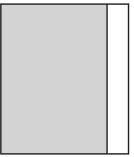
\includegraphics[scale=.4]{Images/fraccion-a.png}
\item 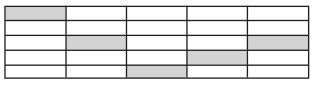
\includegraphics[scale=.4]{Images/fraccion-b.png} 
\item 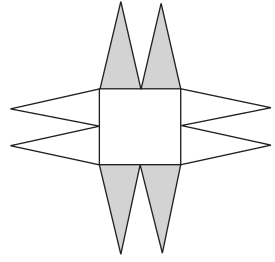
\includegraphics[scale=.4]{Images/fraccion-c.png}
\end{multicols}
\end{enumerate}
\end{enumerate}
\end{document}
